\part[Higher-Order Functions]{Higher-Order Functions}
\section{First-class functions}
\begin{frame}{First-class functions}
\begin{block}{What is a first-class citizen of a programming language?}
\pause
A first-class citizen is an entity that can be constructed at run-rime\\
\end{block}
\pause
\begin{center}
\highlight{First-class citizens are data}
\end{center}
\pause
\begin{block}{What does it mean to be data in a programming language?}
\pause
Data can be:
\begin{itemize}
  \item stored
  \item passed around as an argument for other functions
  \item the result of a function
\end{itemize}
\end{block}
\pause
\begin{block}{What is a first-class function?}
A first-class function is a function, which can be treated as data
\end{block}
\end{frame}

\begin{frame}[fragile]{First-class functions}
\begin{block}{What is a literal?}
\pause
A literal is a way to write a constant value directly in code
\end{block}
\pause
\begin{exampleblock}{Examples}
\begin{lstlisting}
10  // decimal integer literal
20L // decimal long literal
30l // decimal long literal
0x5 // hexadecimal integer literal
035 // octal integer literal
1.2 // double literal
'a' // character literal
'\n' // special character literal
'\u0041' // unicode character literal
"hello"   // string literal
true      // boolean literal
(x: Int, y: Int) => x + y // function literal
\end{lstlisting}
\end{exampleblock}
\end{frame}

\pictureframe{First-class functions' literal syntax}{resources/function.pdf}

\begin{frame}{First-class functions}
\begin{block}{What is an anonymous function?}
\pause
An anonymous function is a function which does not have a name
\end{block}
\pause
\begin{block}{What is a lambda?}
\pause
Lambdas are anonymous functions
\end{block}
\pause
\begin{block}{What is a function literal?}
\pause
A function literal is a way to write an anonymous function value directly in
code
\end{block}
\pause
\begin{block}{What is a function value?}
\pause
A function value is an entity which exists at runtime
\end{block}
\end{frame}

\begin{frame}[fragile]{Playing around with first-class functions}
\begin{lstlisting}
scala> val add = (x: Int, y: Int) => x + y
add: (Int, Int) => Int = <function2>

\end{lstlisting}
\pause
\begin{lstlisting}
scala> val sum = add(2,3)
sum: Int = 5
\end{lstlisting}
\end{frame}

\section{Higher-order functions}
\begin{frame}{Higher-order functions}
\begin{block}{What is a higher-order function/method?}
\pause
A \highlight{higher-order function/method} is a function/method which either
takes \highlight{another function} as an argument or yields a
\highlight{function} as a result or both
\end{block}
\pause
\begin{center}
Higher-order functions/methods need first-class function \highlight{values}, but
not necessarily first-class function \highlight{literals} or lambdas
\end{center}
\end{frame}

\begin{frame}[fragile]{Playing around with higher-order functions}
\begin{exampleblock}{Higher-ordere method \lstinline!foreach!}
\begin{lstlisting}
scala> val numbers = List(1, 2, 3)
numbers: List[Int] = List(1, 2, 3)
\end{lstlisting}
\pause
\begin{lstlisting}
scala> val show = (x: Int) => println(x)
show: Int => Unit = <function1>
\end{lstlisting}
\pause
\begin{lstlisting}
scala> numbers.foreach(show)
1
2
3
\end{lstlisting}
\end{exampleblock}
\end{frame}

\begin{frame}[fragile]{Syntactic sugar for syntactic sugar}
\begin{lstlisting}
numbers.foreach((x: Any) => println(x))
\end{lstlisting}
\pause
\begin{lstlisting}
numbers.foreach((x) => println(x))
\end{lstlisting}
\pause
\begin{lstlisting}
numbers.foreach(x => println(x))
\end{lstlisting}
\pause
\begin{lstlisting}
numbers.foreach(println(_))
\end{lstlisting}
\pause
\begin{lstlisting}
numbers.foreach(println _)
\end{lstlisting}
\pause
\begin{lstlisting}
numbers.foreach(println)
\end{lstlisting}
\pause
\begin{lstlisting}
numbers foreach println
\end{lstlisting}
\end{frame}

\begin{frame}[fragile]{Playing around with higher-order functions}
\begin{lstlisting}
scala> val numbers = List(-10, -5, 0, 5, 10)
numbers: List[Int] = List(-10, -5, 0, 5, 10)
\end{lstlisting}
\pause
\begin{lstlisting}
scala> val filteredNumbers = numbers.filter(_ > 0)
filteredNumbers: List[Int] = List(5, 10)
\end{lstlisting}
\pause
\begin{lstlisting}
scala> val sortedNumbers = filteredNumbers.sortWith(_ > _)
sortedNumbers: List[Int] = List(10, 5)
\end{lstlisting}
\pause
\begin{lstlisting}
scala> sortedNumbers.foreach(println)
10
5
\end{lstlisting}
\end{frame}

\begin{frame}[fragile]{Playing around with higher-order functions}
\begin{exampleblock}{What is printed out?}
\begin{tabular}{l|l}
\begin{lstlisting}
List(-10, -5, 0, 5, 10)
  .filter(_ > 0)
  .map(x => x * x)
  .sortWith(_ > _)
  .foreach(println)
\end{lstlisting}
&
\begin{lstlisting}
List(-10, -5, 0, 5, 10)
  .map(x => x * x)
  .filter(_ > 0)
  .sortWith(_ > _)
  .foreach(println)
\end{lstlisting}\\
\hline
\pause
\begin{lstlisting}
100
25
\end{lstlisting}
&
\begin{lstlisting}
100
100
25
25
\end{lstlisting}
\end{tabular}
\end{exampleblock}
\end{frame}

\section{Closures}
\begin{frame}[fragile]{Closures}
\begin{block}{What is a closed term?}
A closed term is a function \alert{without} free variables
\end{block}
\pause
\begin{exampleblock}{Closed term}
\lstinline!(a: Int) => a + 1!
\end{exampleblock}
\pause
\begin{block}{What is an open term?}
An open term is a function \highlight{with} free variables
\end{block}
\pause
\begin{exampleblock}{Open term}
\lstinline!(a: Int) => a + x!
\end{exampleblock}
\pause
\begin{block}{What is a closure?}
A closure is the function value of the open term, thus a closure closes the open
term at runtime, by capturing the bindings of its free variables
\end{block}
\end{frame}

\begin{frame}{Closures}
\begin{center}
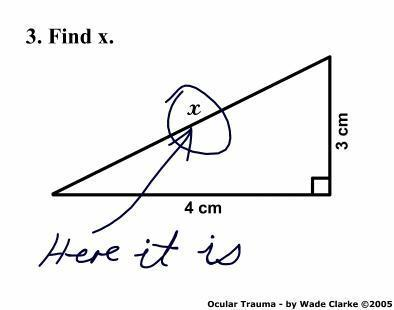
\includegraphics{resources/FindX.jpg}
\end{center}
\end{frame}

\begin{frame}[fragile]{Closures}
\begin{exampleblock}{\lstinline!x! has to be in the context of the function}
\begin{lstlisting}
scala> val x = 10
x: Int = 10
\end{lstlisting}
\pause
\begin{lstlisting}
scala> val closure = (a: Int) => a + x
closure: Int => Int = <function1>
\end{lstlisting}
\pause
\begin{lstlisting}
scala> val sum = closure(20)
sum: Int = 30
\end{lstlisting}
\end{exampleblock}
\end{frame}

\section{Function currying}
\begin{frame}[fragile]{Function currying}
\pause
\begin{exampleblock}{Bringing \lstinline!x! closer to the scope of the function}
\begin{lstlisting}
scala> def getClosure(x: Int) = (a: Int) => a + x
getClosure: (x: Int)Int => Int
\end{lstlisting}
\pause
\begin{lstlisting}
scala> val closure = getClosure(10)
closure: Int => Int = <function1>
\end{lstlisting}
\pause
\begin{lstlisting}
scala> val sum = closure(20)
sum: Int = 30
\end{lstlisting}
\pause
\begin{lstlisting}
scala> val sum = getClosure(10)(20)
sum: Int = 30
\end{lstlisting}
\end{exampleblock}
\end{frame}

\begin{frame}{Function currying}
\begin{block}{What is a curried function?}
A curried function is applied to multiple argument lists, instead of just one
\end{block}
\end{frame}

\begin{frame}[fragile]{Function currying}
\begin{exampleblock}{Syntactic sugar for function currying}
\begin{lstlisting}
scala> def getClosure(x: Int)(a: Int) = a + x
getClosure: (x: Int)(a: Int)Int
\end{lstlisting}
\pause
\begin{lstlisting}
scala> val closure = getClosure(10)(_)
closure: Int => Int = <function1>
// or alternatively
scala> val closure = getClosure(10) _
closure: Int => Int = <function1>

scala> val sum = closure(20)
sum: Int = 30

scala> val sum = getClosure(10)(20)
sum: Int = 30
\end{lstlisting}
\end{exampleblock}
\end{frame}

\section{Magic behind the scenes}
\begin{frame}{Function values are objects}
\begin{block}{What is a first-class citizen of a programming language?}
\pause
A first-class citizen is an entity that can be constructed at run-rime
\end{block}
\pause
\begin{block}{What is a runtime entity in an OO environment?}
\pause
A runtime entity is an object
\end{block}
\pause
\begin{center}
\highlight{Function values are objects}
\end{center}
\end{frame}

\begin{frame}{Function values are objects}
A \highlight{function literal} is compiled into a \highlight{class} that when
instantiated at runtime is a function value. Every function value is an instance
of some (anonymous) class that extends one of several \lstinline!FunctionN!
traits in package scala, such as \lstinline!Function0! for functions with no
parameters, \lstinline!Function1! for functions with one parameter, and so on.
Each \lstinline!FunctionN! trait has an \lstinline!apply! method used to invoke
the function.
\end{frame}

\begin{frame}[fragile]{FunctionN traits}
\begin{block}{\lstinline!Function2!}
\begin{lstlisting}
trait Function2[-T1, -T2, +R] extends AnyRef {
   def apply (v1: T1, v2: T2): R 
   ...
}
\end{lstlisting}
\end{block}
\pause
\begin{exampleblock}{\lstinline!FunctionName!}
\begin{lstlisting}
class FunctionName extends Function2[Int, Int, Int] {
   def apply(a: Int, b: Int): Int = a + b
} 
\end{lstlisting}
\end{exampleblock}
\end{frame}

\begin{frame}[fragile]{FunctionN traits}
\begin{exampleblock}{Using \lstinline!FunctionName!}
\begin{lstlisting}
val add = new FunctionName
val sum = add.apply(10, 20)
// scalac infers calls to apply
val sum = add(10, 20)
\end{lstlisting}
\end{exampleblock}
\pause
\begin{alertblock}{Inlining \lstinline!FunctionName! (does not compile)}
\lstinline!val sum = new FunctionName(2, 3)!
\end{alertblock}
\pause
\begin{block}{Inlining \lstinline!FunctionName! (not idiomatic scala)}
\lstinline!val sum = new FunctionName()(2, 3)!
\end{block}
\pause
\begin{exampleblock}{Inlining \lstinline!FunctionName!}
\lstinline!val sum = (new FunctionName)(2, 3)!
\end{exampleblock}
\end{frame}

\begin{frame}[fragile]{Function literals are call-backs}
\begin{block}{The name of \lstinline!FunctionName! is unessential}
\begin{lstlisting}
val add = new Function2[Int, Int, Int] {
   def apply(a: Int, b: Int) = a + b
} 
\end{lstlisting}
\end{block}
\pause
\begin{exampleblock}{Function literals are syntactic sugar for anonymous
call-backs}
\begin{lstlisting}
val add = ((a, b) => a + b): Function2[Int, Int, Int]
val add = ((a, b) => a + b): (Int, Int) => Int
val add: Function2[Int, Int, Int] = (a, b) => a + b
val add: ((Int, Int) => Int) = (a, b) => a + b
val add: ((Int, Int) => Int) = _ + _
val add = (a: Int, b: Int) => a + b
val add = (_: Int, _: Int) => _ + _
\end{lstlisting}
\end{exampleblock}
\end{frame}

\begin{frame}[fragile]{Closures}
\begin{exampleblock}{No sugar}
\begin{lstlisting}
val x = 10
val closure = new Function1[Int, Int] {
   def apply(a: Int) = a + x
}
val sum = closure(20) // 30
\end{lstlisting}
\end{exampleblock}
\begin{exampleblock}{Some sugar}
\begin{lstlisting}
val x = 10
val closure = (a: Int) => a + x
val sum = closure(20) // 30
\end{lstlisting}
\end{exampleblock}
\end{frame}

\begin{frame}[fragile]{Currying}
\begin{exampleblock}{No sugar}
\begin{lstlisting}
def getClosure(x: Int) = new Function1[Int, Int] {
   def apply(a: Int) = a + x
}
\end{lstlisting}
\end{exampleblock}
\begin{exampleblock}{Some sugar}
\lstinline!def getClosure(x: Int) = (a: Int) => a + x!
\end{exampleblock}
\begin{exampleblock}{Lots of sugar}
\lstinline!def getClosure(x: Int)(a: Int) = a + x!
\end{exampleblock}
\end{frame}

\section{Summary}
\begin{frame}{Summary}
\begin{itemize}
  \item Function \highlight{literals} are constant values in \highlight{source
  code}
  \item Function \highlight{values} are objects at \highlight{runtime}
  \item \highlight{Lambdas} are \highlight{anonymous} functions
  \item \highlight{First-class functions} are functions, which are treated as
  data
  \item \highlight{Higher-order functions} are functions, which take
  \highlight{first-class functions} as arguments or yield functions as results
  \item \highlight{Closures} are functions with free variables
  \item \highlight{Curried functions} are applied to multiple argument lists,
  instead of just one
  \item Function literals are just syntactic sugar for \highlight{anonymous
  classes}
  \item Don't get a sugar rush ;)
\end{itemize}
\end{frame}